\documentclass{beamer}

\usepackage[british]{babel}
\usepackage{graphicx,hyperref,tue,url}
\usepackage{amsmath}

% The title of the presentation:
%  - first a short version which is visible at the bottom of each slide;
%  - second the full title shown on the title slide;
\title[Network\_science]{
  Link Prediction:\\ 
  Similarity Indexes}
  %What is it and how to tackle it? }

%\subtitle{Similarity Indexes}

% The author(s) of the presentation:
%  - again first a short version to be displayed at the bottom;
%  - next the full list of authors, which may include contact information;
\author[Andrea Mangrella]{
  Andrea Mangrella\\
  Roëlle Bänffer\\
  Maarten van Sluijs\\
  }

% The institute:
%  - to start the name of the university as displayed on the top of each slide
%    this can be adjusted such that you can also create a Dutch version
%  - next the institute information as displayed on the title slide
\institute[Eindhoven University of Technology]{
  Department of Mathematics and Computer Science \\
  Eindhoven University of Technology}

% Add a date and possibly the name of the event to the slides
%  - again first a short version to be shown at the bottom of each slide
%  - second the full date and event name for the title slide
\date[slides Example 2012]{
    9th October 2023   
  }

\begin{document}

\begin{frame}
  \titlepage
\end{frame}

\begin{frame}
  \frametitle{Outline}
  \tableofcontents
\end{frame}

% INTRODUCTION:
\section{Introduction}
\begin{frame}
  \frametitle{Introduction}
  Link prediction is the act of finding relevant novel or missing connections in a network.\\
  \vspace{1cm}
  Various applications of link prediction include:
  \begin{itemize}
      \item Recommender systems for streaming services or social networks apps.
      \item To aid in identifying possible avenues of research:
      \begin{itemize}
          \item Protein-protein interactions
          \item Metabolic networks.
      \end{itemize}
  \end{itemize}
\end{frame}

\begin{frame}
  \frametitle{Introduction}
  Similarity based link prediction:
  \begin{columns}
    % column 1
    \begin{column}{6.5cm}
        \quad \quad Some graph $G = (V,E)$\\
        \quad \quad All possible edges given by $U = \binom{n}{2}$\\
        \quad \quad All non-edges are $N = U - E$
    \end{column}
    % Column 2
    \begin{column}{3cm}
    \begin{centering}
    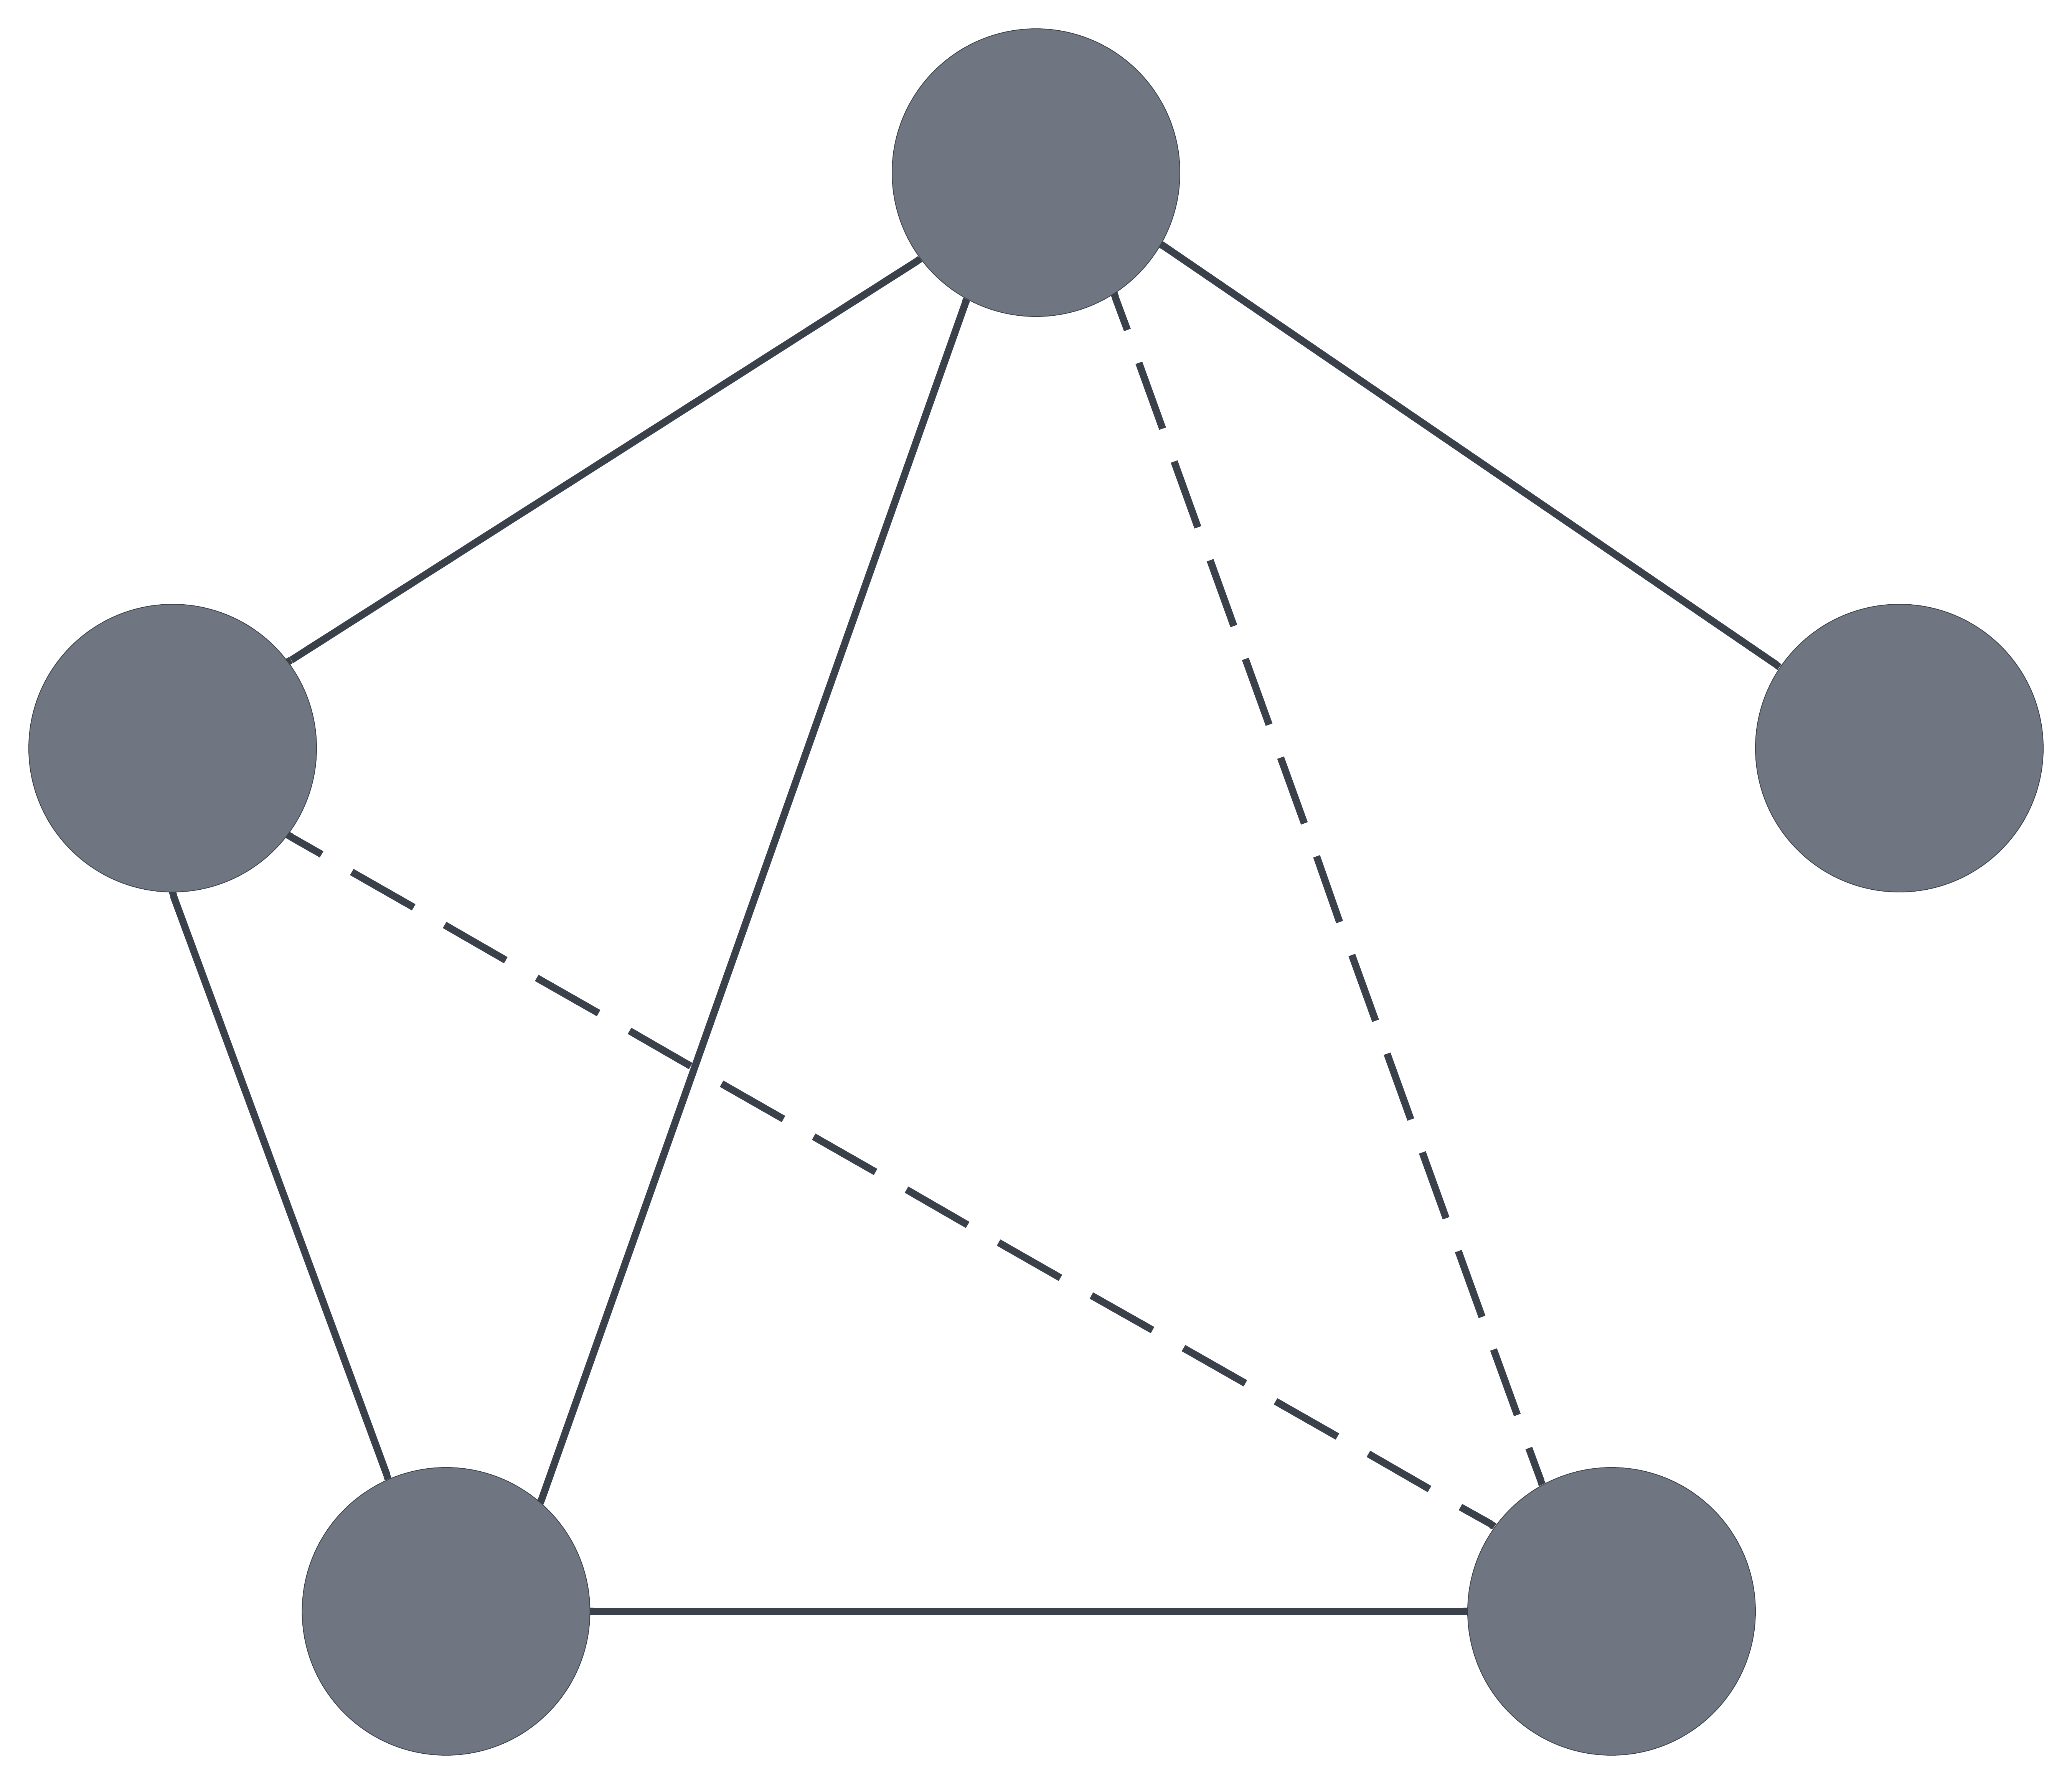
\includegraphics[width=4cm]{Link prediction.png}
  \end{centering}
    \end{column}
\end{columns}
Define some similarity: $s_{xy} = f(x,y)$\\
Rank edges $e_{xy}\in N$ based on this score $s_{xy}$. 
\end{frame}

\section{Testing and Metrics}
\begin{frame}
  \frametitle{Testing the Indices}
To test the algorithm’s \textbf{Accuracy}, the observed links, E, are randomly divided into two parts: the \textbf{Training set} and the \textbf{Probe set}. \\%(\bold{E^T} and   \bold{E^P}). 
\smallskip
\color{purple}Disadvantage: \color{black} some link may \textbf{never be selected} in the probe set, and other may be selected many times.
\end{frame}

\begin{frame}
  \frametitle{Testing the Indices}
To test the algorithm’s \textbf{Accuracy}, the observed links, E, are randomly divided into two parts: the \textbf{Training set} and the \textbf{Probe set}. \\%(\bold{E^T} and   \bold{E^P}). 
\smallskip
\color{purple}Disadvantage: \color{black} some link may \textbf{never be selected} in the probe set, and other may be selected many times.\\
\medskip
\color{teal}Solution: \color{black} use k-cross validation, in which the edges get partitioned in \textbf{k} subset. The process is repeated k times to use \emph{\textbf{every subset as the probe set}}.
\end{frame}
\begin{frame}
  \frametitle{Testing Metrics}
  \emph{\textbf{Accuracy}}: is the ratio of relevant items
to the number of selected item. The result unfortunately focuses only on the top L candidates\\
    \[Precision = \dfrac{l}{L}\] \\
  \bigskip 
  \emph{\textbf{AUC}}: the probability that a randomly chosen missing link (a link in EP) is given a higher score than a randomly chosen nonexistent link.The result is the overall ranking resulted from the algorithm. \\
   \[AUC = \dfrac{n' + 0.5n''}{n}\]
\end{frame}

%Local Similarity Indices:
\section{Local Similarity Indices}
\begin{frame}
\frametitle{Local Similarity Indices}
Local indices are generally calculated using information about common neighbours and node degree. These indices consider \textbf{immediate neighbours of a node}.\\
\bigskip
\textbf{Common Neighbours:} \\
For a node x $\Gamma_{x}$ is the set of neighbours of x. The simplest measure for similarity is then the neighborhood overlap between two nodes x and y.
\[s^{CN}_{xy} = |\Gamma_{x} \cap \Gamma_{y}| \]
\end{frame}

\begin{frame}
\bigskip
Variations of the Common Neighbour method: \\
\bigskip
\textbf{Salton Index:} $s^{Salton}_{xy} = \dfrac{|\Gamma_{x} \cap \Gamma_{y}|}{\sqrt{k_{x} \times k_{y}}}$ (Cosine Similarity)\\
\bigskip
\textbf{Jaccard Index:}  $s^{Jaccard}_{xy} = \dfrac{|\Gamma_{x} \cap \Gamma_{y}|}{|\Gamma_{x} \cup \Gamma_{y}|}$\\
\bigskip
\textbf{Leight-Holme-Newman Index:}  $s^{LHN1}_{xy} = \dfrac{|\Gamma_{x} \cap \Gamma_{y}|}{k_{x} \times k_{y}}$ \\
\begin{itemize}
    \item Assign high similarity to pairs that have a high expected number of neighbours 
    \item Where $k_{x} \times k_{y}$ is proportional to the number of common neighbours of node x and y in an instance of the Configuration Model.
\end{itemize}
\end{frame}

\begin{frame}
\textbf{Preferential Attachment Index:} $s^{PA}_{xy} = k_{x} \times k_{y}$ \\
\begin{itemize}
    \item This index is based on the mechanism of \textbf{Preferential Attachment}  where the probability that a new link is connected to x is based on is \textbf{degree}. 
    % Prefential Attachment can be used to generate scale free networks,
\end{itemize}
\smallskip
\textbf{Adamic-Adar Index:}  $s^{AA}_{xy} = \sum_{z\in\Gamma_{x} \cap \Gamma_{y}}^{} \dfrac{1}{log(k_{z})}$\\
\begin{itemize}
    \item Simply \textbf{counting of common neighbours} and assigning the less connected neighbours more weight. 
\end{itemize}
\smallskip
\textbf{Resource Allocation Index:}  $s^{RA}_{xy} = \sum_{z\in\Gamma_{x} \cap \Gamma_{y}}^{} \dfrac{1}{k_{z}}$\\
\begin{itemize}
    \item Based on resource allocations dynamics on Complex newtorks.
\end{itemize}
\end{frame}

% Table of metrics 
\begin{frame}
\frametitle{Local Indices Comparison (AUC)}
\begin{figure}
  \centering
  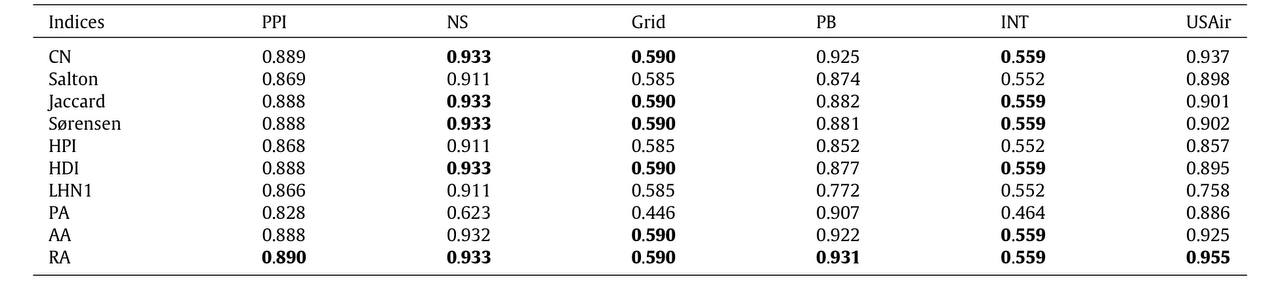
\includegraphics[width=1\linewidth]{andrea_images/table1.jpg}
  \label{fig:table1}
\end{figure}
\end{frame}



% Global Similarity Indices
% Global similarity indices, in contrast to local similarity indices, are path-dependent and global knowledge of the network topology is required. 
\section{Global Similarity Indices}
\begin{frame}
  \frametitle{Global Similarity Indices: Katz Index}
    \[S(x,y) = \sum_{l=1}^{\infty} \beta^{l} |paths_{x,y}^{(l)}| = \sum_{l=1}^{\infty} \beta^{l}(A^{l})_{x,y}\]
    $paths_{x,y}^{(l)}$ is the set of total $l$ length paths between x and y\\
    $\beta$ is the damping factor that controls the path weights

\begin{figure}
\centering
  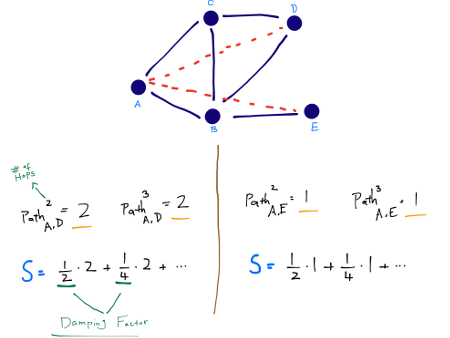
\includegraphics[width=.6\linewidth]{katz-graph.png}
  \label{fig:katz-graph}
\end{figure}

\end{frame}



\begin{frame}
  \frametitle{Global Similarity Indices: Random Walk with Restart (RWR)} 
    \[q_{x}^{\rightarrow} = (1 - \alpha)(I - \alpha P^{T})^{-1}e_{x}^{\rightarrow}\]
    $q_{xy}$ is the probability that a random walker who starts walking from x and located at y\\
    $e_{x}^{\rightarrow}$ is seed vector of length $|V|$ (total number of vertices in graph)
    \begin{align}
P_{xy} =
    \begin{cases}
      1/k_{x}, & \text{if x and y are connected,} \\
      0, & \text{otherwise}
    \end{cases}\\
\begin{cases}
      Prob = \alpha, & \text{go to random neighbor}\\
      Prob = 1 - \alpha, & \text{return to node x}
    \end{cases}
\end{align}
    \[S(x,y) = q_{xy} + q_{yx}\]

\end{frame}

\begin{frame}
  \frametitle{Global Similarity Indices: Shortest Path} 
    Score(x,y) = (negated) Length of shortest path between x and y
    \[S(x,y) = -|d(x,y)|\]
    apply Dijkstra algorithm $\rightarrow$ small world property
    
\begin{figure}
\centering
  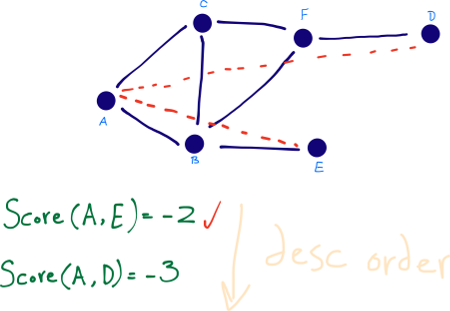
\includegraphics[width=.6\linewidth]{graph-distance-graph.png}
  \label{fig:shortest_path}
\end{figure}
   
\end{frame}


\begin{frame}
  \frametitle{Global Similarity Indices} 
    \textbf{Leicht-Holme-Newman Global Index (LHNG)}
    \[S(x,y) = 2\alpha \lambda_{1}D^{-1}(I-\frac{\beta}{\lambda_{1}}A)^{-1}D^{-1}\]
    D is the matrix $diag(d1,d2,\cdot\cdot\cdot)$\\
    $\lambda_{1}$ is the largest eigenvalue of adjacency matrix A
    \\
    \textbf{Cosine based on $L^{+}$ $(Cos^{+})$}
    \[S(x,y) = \dfrac{l_{x,y}^{+}}{\sqrt{l_{x,x}^{+} l_{y,y}^{+}}}\]
    Inner product measure that uses cosine similarity\\
    Use SVD to get $\rightarrow$ inner products of the node vectors $l_{xy}^{+} = v_{x}^{T}v_{y}$
\end{frame}

\begin{frame}
  \frametitle{Global Similarity Indices}
    \textbf{Average Commute Time (ACT)}
    \[S(x,y) = \dfrac{1}{l_{xx}^{+} + l_{yy}^{+} - 2l_{xy}^{+}}\]
    $l_{xy}^{+}$ is an entry in $L^{+} (L=D-A)$
    average number of steps by random walker from node x to node y\\
    \textbf{Normalized Average Commune Time (NACT)}
    \[S(x,y) = \dfrac{1}{(m(x,y)\pi_{y} + m(y,x)\pi_{x})}\]
\end{frame}

\begin{frame}
  \frametitle{Global Similarity Indices}
    \textbf{Matrix Forest Index (MF)}
    \[S = (I + L)^{-1}\]
    $(I+L)_{(x,y)}$ is number of spanning rooted forests\\
    Uses spanning trees that contain both nodes x and y
\begin{figure}
  \centering
  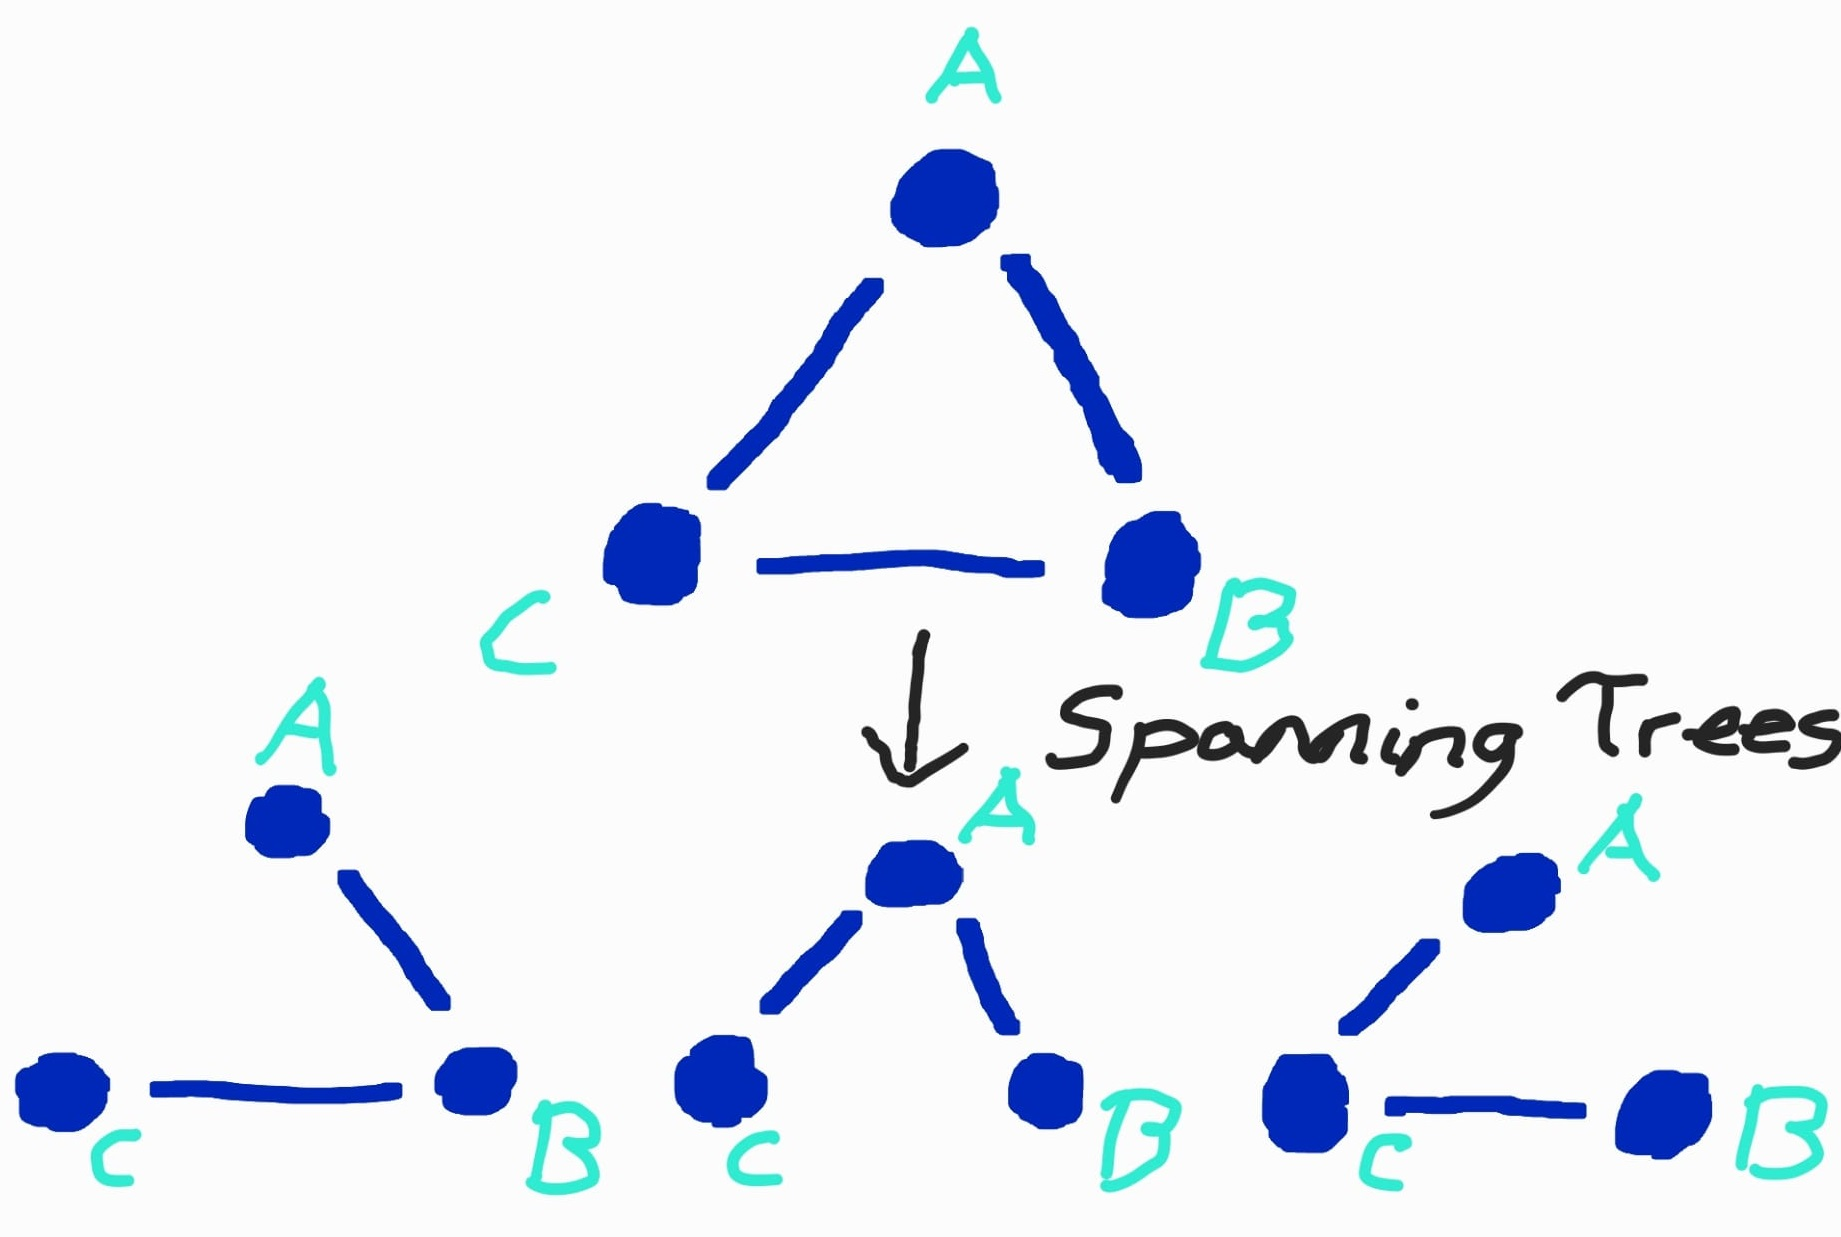
\includegraphics[width=.5\linewidth]{spanning_trees.jpg}
  \label{fig:spanning_trees}
\end{figure}
\end{frame}

\begin{frame}
  \frametitle{Global Similarity Indices}
    \textbf{SimRank}
    \[S(x,y) = \alpha W^{T}SW + (1 - \alpha)I\]
    W is the transformation matrix and computed by normalizing each column of adjacency matrix A
    Structural context similarity and object-to-object relationships\\
    Assumption: two objects are similar if they are related to similar objects\\
    Two random walkers start from different positions\\
\end{frame}

\begin{frame}
  \frametitle{Global Similarity Indices}
    \textbf{Rooted Pagerank (RPR)}
    \[RPR = (1 - \alpha)(I - \alpha \^{N})^{-1}\]
    $\^{N} = D^{-1}A$ is the normalized adjacency matrix with the diagonal degree matrix $D[i,i] = \sum_{j}A[i,j]$\\

    \begin{cases}
      $Prob = \alpha$, & \text{go to random neighbor}\\
      $Prob = 1 - \alpha$, & \text{return to node x}
    \end{cases}
\end{frame}

% Quasi-local Similarity Indices
\section{Quasi-local Similarity Indices}
\begin{frame}
  \frametitle{Quasi-local Similarity Indices}
Quasi-local Similarity indices have been introduced as a \textbf{trade-off} between  \emph{\textbf{Performance}} and \emph{\textbf{Complexity}} (local and global approaches). \\
\bigskip
  \textbf{Local Path Index (LP)}
  \[S^{LP} = A^{2} + \varepsilon A^{3} + \varepsilon^{2} A^{4} + ... \varepsilon^{n-2} A^{n}\]
  \begin{itemize}
      \item $\varepsilon$ is free parameter (if set to 0 the algorithm works as CN)\\
      \item $(A^{n})_{xy}$ is equal number of different paths with length \emph{n} connecting \emph{x} and \emph{y}\\
  \end{itemize} 
\end{frame}

\begin{frame}
  \frametitle{Random Walk }
  Random Walk is a Markow Chain describing the sequence of nodes visited by a random walker. It can be described using the matrix P in where $P_{xy}$ (the probability x will go to y) is defined as: \\
  \[P_{xy}=\dfrac{a_{xy}}{k_{x}}\] 
  \begin{itemize}
      \item $k_{x}$ is the degree of the node 
      \item $a_{xy}$ describes if an edge between x and y is present (1) or not (0)
  \end{itemize}
\end{frame}

\begin{frame}
  \frametitle{Random Walk}
  Given a random walker starting from node x we define the probability that the walker locates at node y after t steps as: \\
  \[\pi_{xy}(t)\]
  \bigskip
  Then we can say: 
  \[\pi_{x}(t)=P^{T}\pi_{x}(t-1)\]
  
\end{frame}

\begin{frame}
  \frametitle{Local Random Walk}
  \textbf{LRW}: \\
  \[s_{xy}^{LRW}(t) =\dfrac{k_{x}}{2|E|}\pi_{xy}(t) + \dfrac{k_{y}}{2|E|}\pi_{yx}(t)\]\\
  \bigskip
  \bigskip
  
  \color{red}\ench{\textbf{Disadvantage: }}\color{black} unfortunately the metric is sensitive to the rest of the network that is distant from x and y (i.e. not every time uses the shortest path between the 2 nodes).\\
\end{frame}

\begin{frame}
  \frametitle{Superposed Random Walk}
  \textbf{SRW}:\\ 
  A possible solution to the LRW problem, continuously resets walkers to the starting point: \\
  \bigskip
  \[s_{xy}^{LRW}(t) = \sum_{\tau=1}^{t}s_{xy}^{LRW}(\tau)\]
\end{frame}

% Table of metrics 
\begin{frame}
\frametitle{Quasi-Local Indices Comparison}
\begin{figure}
  \centering
  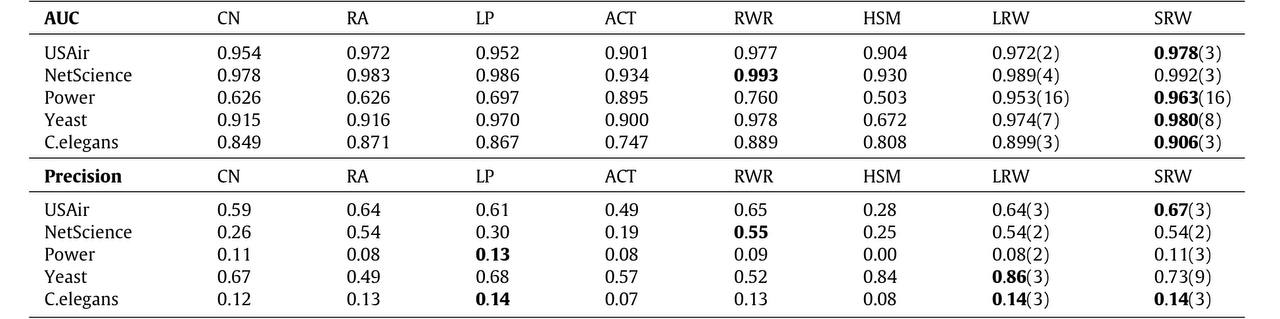
\includegraphics[width=1\linewidth]{andrea_images/table2.jpg}
  \label{fig:table2}
\end{figure}
\end{frame}

% Pros and Cons of Link Prediction 
% Two difficulties in link prediction are the sparsity and huge size of the target networks.
\section{Pros and Cons of Link Prediction}
\begin{frame}
  \frametitle{Pros and Cons of Link Prediction}
  \textbf{Difficulties in link prediction:} 
  \begin{itemize}
      \item Sparsity  \\
      \item Size of target networks \\
  \end{itemize}
  \bigskip
  
\resizebox{10.2cm}{1.2cm}
{
\begin{tabular}{c|ccc}
\hline
    Properties & Local indices & Global indices & Quasi-local indices\\
\hline
    Nature & Simple & Complex & Moderate\\
    Features employed & Local neighborhood & Entire network & More than local neighborhood\\
    Computational complexity & Low & High & Moderate\\
    Parallelization & Easy & More complex & Moderate\\
    Implementation & Feasible for large networks & Feasible for small networks & Feasible for large networks\\
\hline
\end{tabular}
}
  
\end{frame}

\end{document}
    